\section{Experiments}
\label{sec:cod_experimental}
In this section, the performed experiments are going to be described. Specifically, in  
Section~\ref{sec:cod_dataset} the dataset used for training procedure will be described. Section~\ref{sec:cod_results} will report the obtained results.
\subsection{Dataset}
\label{sec:cod_dataset}
To validate the proposed architecture, a simulated dataset was generated, focusing on four primary tasks: \textit{Pick-Place}, \textit{Nut-Assembly}, \textit{Stack-Block}, and \textit{Press-Button}. Each task consists of multiple variations. Specifically, the Pick-Place task has 16 variations, Nut-Assembly has 9 variations, Stack-Block has 6 variations, and Press-Button has 6 variations. Each task and its variations are graphically described in Figure~\ref{fig:dataset_cod}.
\begin{figure}[t]
    \centering
    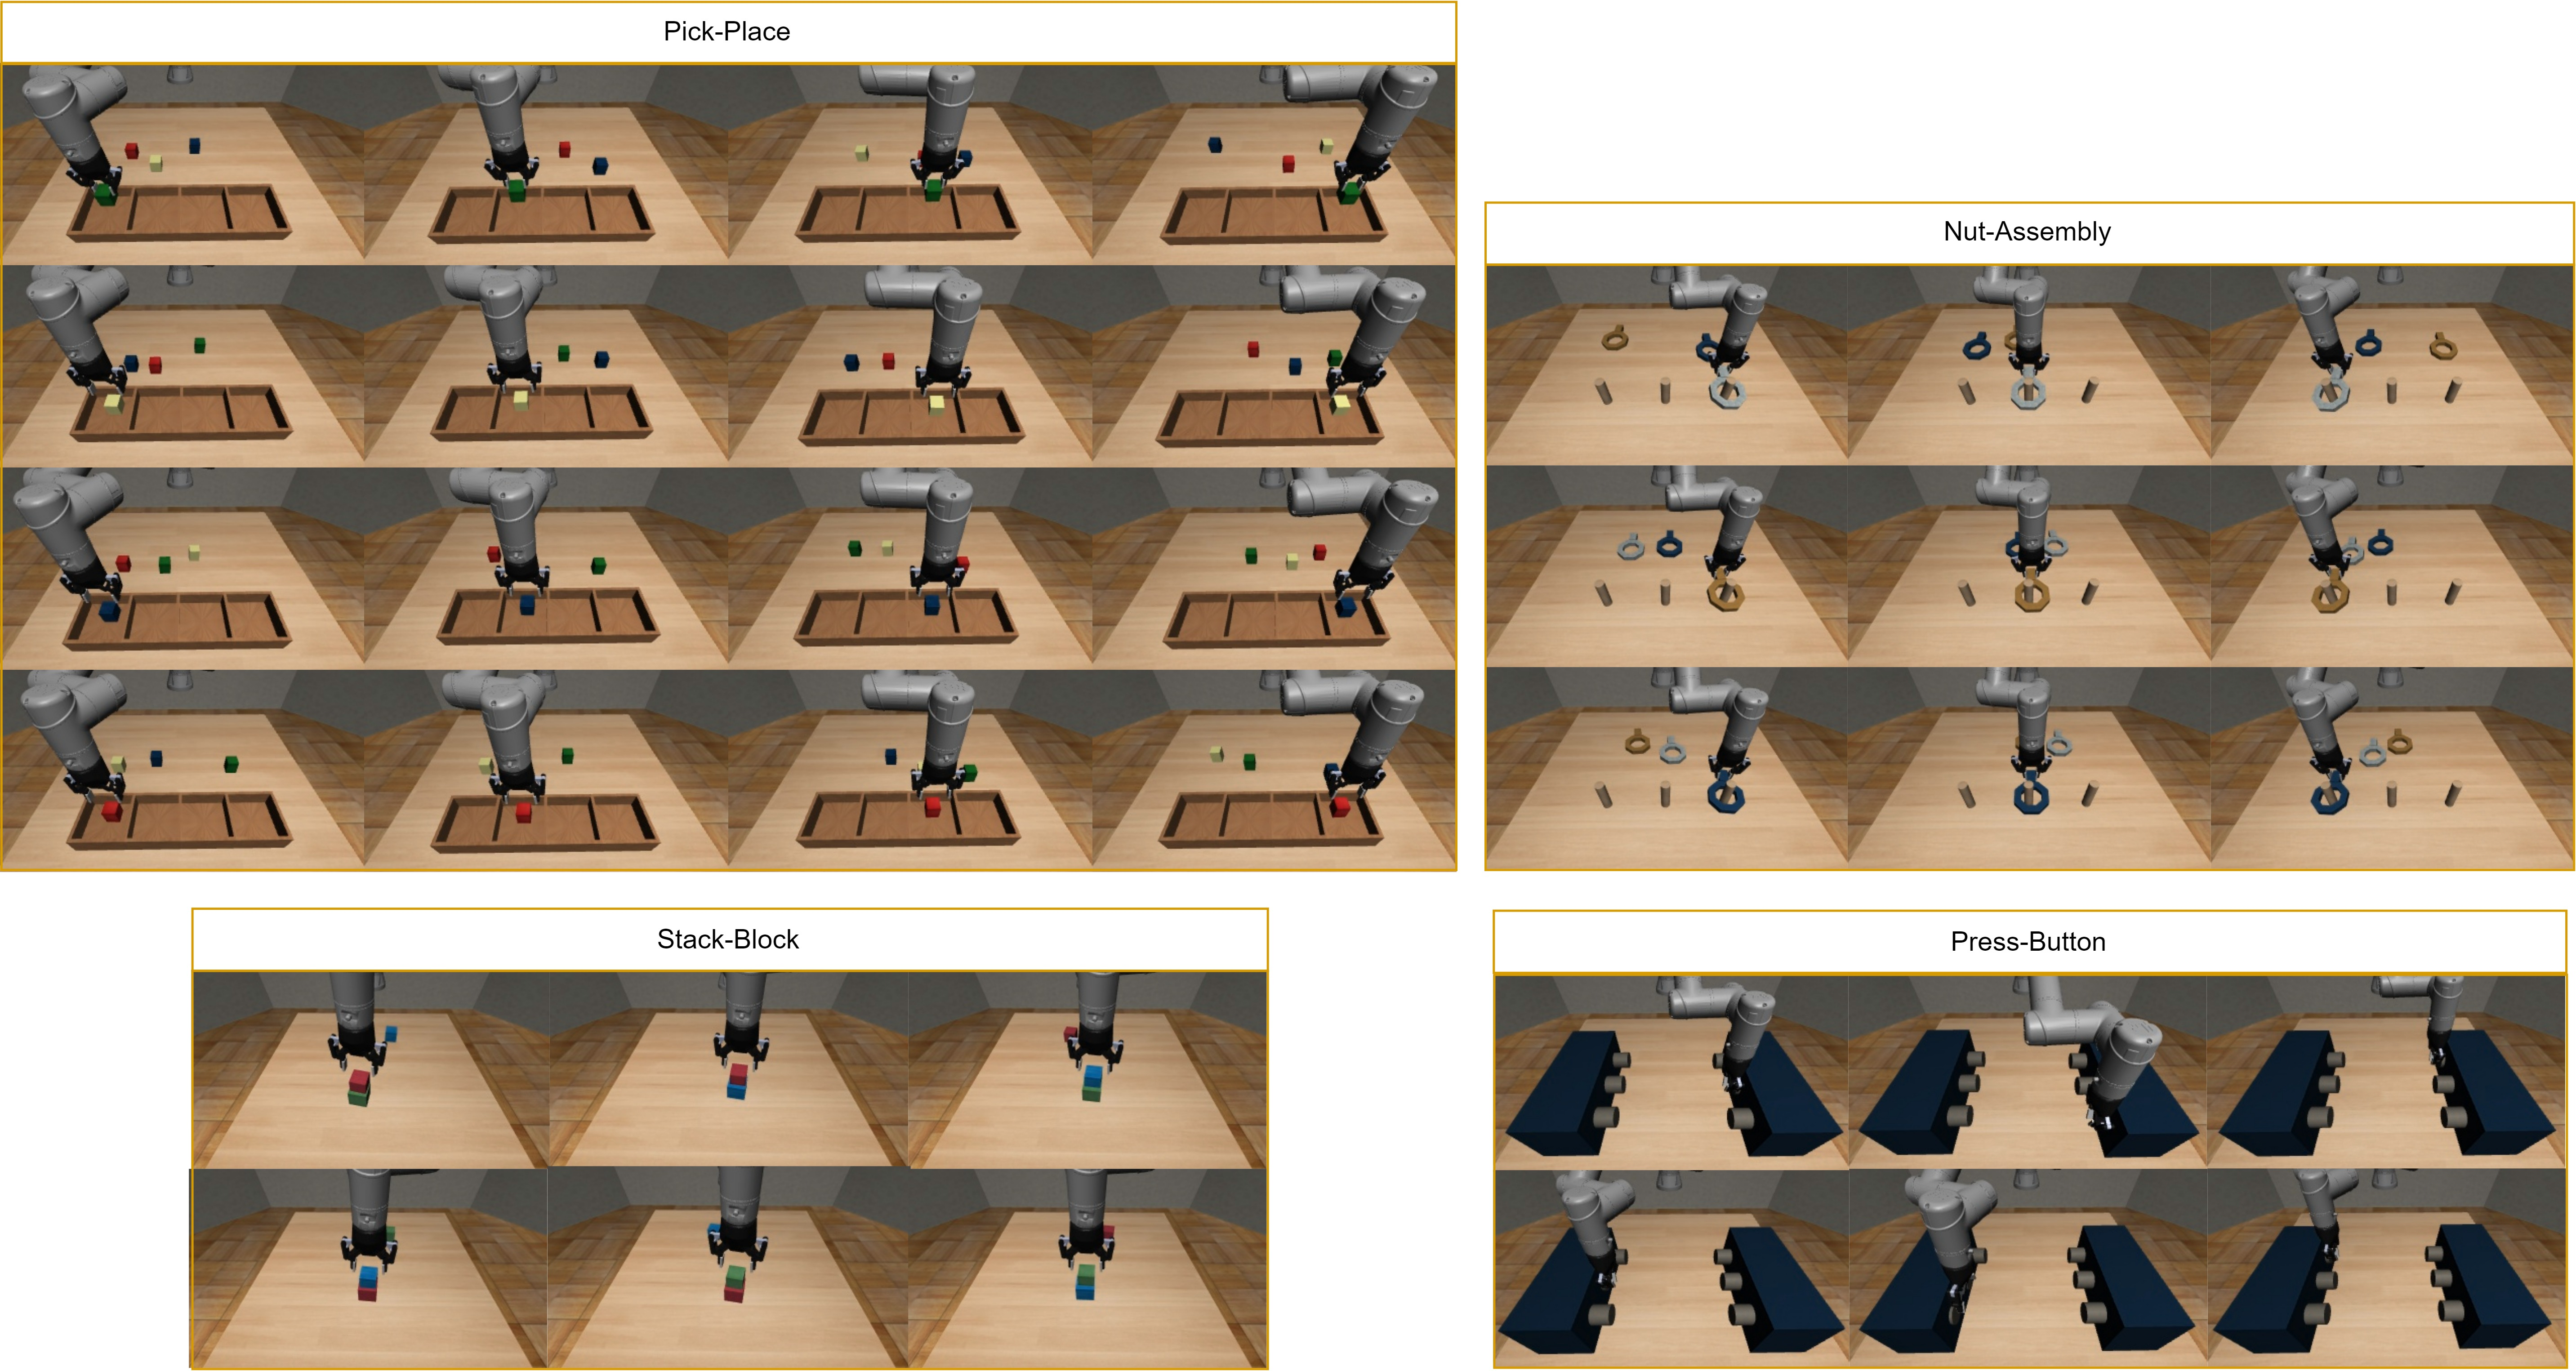
\includegraphics[width=1.0\textwidth]{figures/images/ch2/dataset.jpg}
    \caption{Examples of tasks and variations taken in consideration for the methods validation. The images report the final system state. For the pick-place, nut-assembly and stack-block tasks the variation is defined with respect to the target object and the placing location, while for the press-button the variation is defined according to the button to press.}
    \label{fig:dataset_cod}
\end{figure}


For each task, 100 trajectories were collected for both the agent (UR5e robot) and the demonstrator (Franka-Emika Panda robot) using hand-written policies that take as input ground-truth information about the object position. Across these trajectories, the position of the objects of interest varies. The workspace for each task is divided as follows:
\begin{itemize}
    \item \textbf{Pick-Place}: The bins are fixed in position, while the boxes can change according to the following rule. The workspace is divided into 4 slots, parrallel to the bins, each with a width of $6 \ \text{cm}$ and a height of $15 \ \text{cm}$. A slot is randomly selected, and the box is randomly spawned within the chosen slot, ensuring that each slot is filled with only one object.
    \item \textbf{Nut-Assembly}: The pegs are fixed in position, while the nuts vary in placement. A spawn region of $75 \times 10 \ \text{cm}$ is defined, and the nuts are randomly spawned in this region, ensuring they do not collide with one another.
    \item \textbf{Stack-Block}: The placing box is spawned in a region of $16 \times 5 \ \text{cm}$, while the target box is spawned in a region of $24 \times 5 \ \text{cm}$, ensuring no collisions between the boxes.
    \item \textbf{Press-Button}: The two sets of buttons are placed within a region of $4 \times 4 \ \text{cm}$.
\end{itemize}

The bounding boxes are generated automatically using a procedure that assumes prior knowledge of the object's pose and dimensions, as well as the camera's pose and intrinsic parameters. With this information, a 3D bounding box can be constructed around the object in continuous world space. The corners of this bounding box are then projected into the 2D discrete camera space via a sequence of transformations, as described in Equation \ref{eq:transformation_from_world_to_px}.

\begin{equation}
    \label{eq:transformation_from_world_to_px}
    \begin{matrix}
        \tilde{p}^{camera}_{object} = T^{camera}_{world} \times \tilde{p}^{world}_{object}
        \\ \\
        px_x =  \frac{p_x}{p_z} \cdot f + \frac{w}{2} 
        \\ \\
        px_y =  \frac{p_y}{p_z} \cdot f + \frac{h}{2}
    \end{matrix}
\end{equation}

In this equation, $T^{camera}_{world} \in \mathcal{R}^{4 \times 4}$ represents the homogeneous transformation matrix that defines the camera orientation and position relative to the world frame. The term $\tilde{p}^{src}_{target} = \left[ p_x, p_y, p_z, 1 \right]$ denotes the homogeneous position vector of the \textit{target} frame relative to a given \textit{src} frame. For instance, $\tilde{p}^{world}_{object}$ describes the position of the object relative to the world frame. 

The parameters $w$ and $h$ correspond to the image resolution width and height, respectively. The camera's focal length $f$ is given by $f = \frac{0.5 \times h}{\tan(fov_y)}$, where $fov_y$ is the vertical field of view. Finally, $px_x$ and $px_y$ represent the pixel coordinates obtained in the x and y axes, respectively.

% \smalltodo{add equation}
\subsection{Results}
\label{sec:cod_results}
This section presents the obtained results, divided into two main blocks. The first block (Section~\ref{sec:cod_tod}) discusses the results of the method trained to detect only the target object. The second block (Section~\ref{sec:cod_tofpd}) covers the results of the method trained to detect both the target object and the final (placing) location. For each method, results are reported for two different scenarios: first, where the method is trained in a single-task multi-variation scenario; and second, where the method is trained in a multi-task multi-variation scenario.

For all the test configurations described below, the testing procedure was consistent. Specifically, for each task and its variations, 10 rollouts were performed. During each rollout, the robot was controlled by a hand-written policy, and the predicted bounding box was compared with the ground truth, obtained using the same procedure as described earlier.

The metrics used to evaluate the methods were \textit{Precision@0.5} (Equation \ref{eq:prec}) and \textit{Recall@0.5} (Equation \ref{eq:rec}).
\begin{equation}
    \label{eq:prec}
    Pre = \frac{TP}{TP+FP}
\end{equation} 
\begin{equation}
    \label{eq:rec}
    Rec = \frac{TP}{TP+FN}
\end{equation}

A \textit{True Positive} (TP) sample is defined as a predicted bounding box for the target class with an Intersection over Union (IoU) greater than or equal to 0.5 when compared with the ground-truth bounding box. A \textit{False Positive} (FP) sample is defined as a predicted bounding box for the target class with an IoU less than 0.5. A \textit{False Negative} (FN) sample is defined as a target object for which no bounding box was predicted.

The metrics were computed considering only the target bounding boxes, i.e., the bounding boxes predicted for the target object or the target location. Among all the candidates generated by the network, only the one with the highest predicted class score was considered.


\subsubsection{Target object detector}
This first set of validation tests is related to the training of the COD module in a setting where it must predict the location of the target-object. This means that, with respect to the semantic attributes defined in Section \ref{sec:cod_problem}, the set is restricted to just two classes ``target'' and ``no-target''. In this case, the method will be named \textit{Conditioned Target Object Detector} (CTOD).
\label{sec:cod_tod}
\paragraph*{Single-task multi-variation scenario}\mbox{}\\
In the single-task multi-variation scenario, a specific model was trained for each task described in Figure \ref{fig:dataset_cod}. This approach allows for evaluating the model ability to handle tasks of increasing complexity. Initially, the model is evaluated in a simpler scenario, where it predicts the target position of a specific category of objects (e.g., only boxes in pick-and-place, or only nuts in nut-assembly), thereby limiting variability in object categories.
% \usepackage{graphicx}
% \usepackage{hhline}

% \usepackage{hhline}


% \usepackage{graphicx}
% \usepackage{hhline}


\begin{table}[t]
    \centering
    \caption{Results of the CTOD module obtained in the single-task multi-variation scenario. Performances are reported in terms of \textit{Precision} (Prec), \textit{Recall} (Rec) with an IoU threshold of 0.5 and the Average IoU $(IoU_{avg})$ }
    \label{table:ctod_single_task_performance}
    \begin{tabular}{|c|c|c|c|} 
    \hline
    \textbf{Task} & \textbf{Precision@0.5} & \textbf{Recall@0.5} & $\mathbf{IoU_{avg}}$ \\ 
    \hhline{|====|}
    Pick-Place & 0.770 & 1.00 & 0.628 \\ 
    \hline
    Nut-Assembly & 0.985 & 1.00 & 0.789 \\ 
    \hline
    Stack-Block & 0.995 & 1.00 & 0.848 \\ 
    \hline
    Press-Button & 0.997 & 1.00 & 0.899 \\
    \hline
    \end{tabular}
    \end{table}

% \begin{table}[t]
%     \centering
%     \refstepcounter{table}
%     \caption{Distribution of the predicted bounding boxes generated by the CTOD module in the single-task, multi-variation scenario.}
%     \label{table:ctdo_single_task_prediction_distribution}
%     \resizebox{\linewidth}{!}{%
%     \begin{tabular}{|c|c|c|c|c|c|} 
%     \hline
%     \textbf{Task} & \textbf{TP} & \begin{tabular}[c]{@{}c@{}}\textbf{FP }\\\textbf{pre-picking}\end{tabular} & \begin{tabular}[c]{@{}c@{}}\textbf{FP }\\\textbf{post-picking}\end{tabular} & \begin{tabular}[c]{@{}c@{}}\textbf{FN }\\\textbf{pre-picking}\end{tabular} & \begin{tabular}[c]{@{}c@{}}\textbf{FN }\\\textbf{post-picking}\end{tabular} \\ 
%     \hhline{|======|}
%     \begin{tabular}[c]{@{}c@{}}Pick-Place \\(XXXX)\end{tabular} & XXXX & XXXX & XXXX & XXXX & XXXX \\ 
%     \hline
%     \begin{tabular}[c]{@{}c@{}}Nut-Assembly \\(XXXX)\end{tabular} & XXXX & XXXX & XXXX & XXXX & XXXX \\ 
%     \hline
%     \begin{tabular}[c]{@{}c@{}}Stack-Block\\(XXXX)\end{tabular} & XXXX & XXXX & XXXX & XXXX & XXXX \\ 
%     \hline
%     \begin{tabular}[c]{@{}c@{}}Press-Button\\(XXXX)\end{tabular} & XXXX & XXXX & XXXX & XXXX & XXXX \\
%     \hline
%     \end{tabular}
%     }
%     \end{table}

\begin{table}[t]
\centering
\caption{Results of the CTOD module obtained in the multi-task multi-variation scenario. Performances are reported in terms of \textit{Precision} (Prec), \textit{Recall} (Rec) with an IoU threshold of 0.5 and the Average IoU $(IoU_{avg})$}
\label{table:ctod_multi_task_performance}
\begin{tabular}{|c|c|c|c|} 
\hline
\textbf{Task} & \textbf{Precision@0.5} & \textbf{Recall@0.5} & $\mathbf{IoU_{avg}}$ \\ 
\hhline{|====|}
Pick-Place & 0.652 & 1.00 & 0.563 \\ 
\hline
Nut-Assembly & 0.948 & 1.00 & 0.726 \\ 
\hline
Stack-Block & 0.894 & 1.00 & 0.708 \\ 
\hline
Press-Button & 0.977 & 1.00 & 0.825 \\
\hline
\end{tabular}
\end{table}

% \begin{table}[t]
%     \centering
%     \refstepcounter{table}
%     \caption{Distribution of the predicted bounding boxes generated by the CTOD module in the multi-task, multi-variation scenario.}
%     \label{table:ctdo_multi_task_prediction_distribution}
%     \resizebox{\linewidth}{!}{%
%     \begin{tabular}{|c|c|c|c|c|c|} 
%     \hline
%     \textbf{Task} & \textbf{TP} & \begin{tabular}[c]{@{}c@{}}\textbf{FP }\\\textbf{pre-picking}\end{tabular} & \begin{tabular}[c]{@{}c@{}}\textbf{FP }\\\textbf{post-picking}\end{tabular} & \begin{tabular}[c]{@{}c@{}}\textbf{FN }\\\textbf{pre-picking}\end{tabular} & \begin{tabular}[c]{@{}c@{}}\textbf{FN }\\\textbf{post-picking}\end{tabular} \\ 
%     \hhline{|======|}
%     \begin{tabular}[c]{@{}c@{}}Pick-Place \\(XXXX)\end{tabular} & XXXX & XXXX & XXXX & XXXX & XXXX \\ 
%     \hline
%     \begin{tabular}[c]{@{}c@{}}Nut-Assembly \\(XXXX)\end{tabular} & XXXX & XXXX & XXXX & XXXX & XXXX \\ 
%     \hline
%     \begin{tabular}[c]{@{}c@{}}Stack-Block\\(XXXX)\end{tabular} & XXXX & XXXX & XXXX & XXXX & XXXX \\ 
%     \hline
%     \begin{tabular}[c]{@{}c@{}}Press-Button\\(XXXX)\end{tabular} & XXXX & XXXX & XXXX & XXXX & XXXX \\
%     \hline
%     \end{tabular}
%     }
%     \end{table}
Table \ref{table:ctod_single_task_performance} presents the overall performance of the CTOD module in terms of Precision and Recall, providing a comprehensive evaluation of the system ability to accurately identify target objects (Precision) and consistently detect them across multiple rollouts (Recall). The results demonstrate that the module successfully identifies target objects with precise bounding boxes and maintains a high level of consistency across rollouts, achieving excellent precision and recall metrics. 

In particular, the Recall remains consistently at \textbf{1.00}, indicating the absence of false negatives, meaning the system always generates a bounding box classified as the ``target" object. Precision values are also high, exceeding \textbf{0.90} for three tasks: Nut-Assembly, Stack-Block, and Press-Button. However, a lower Precision is observed for the Pick-Place task. This is due to the task longer motion duration, both in terms of time and space, which introduces varying scales of the target object throughout the motion, increasing the complexity of predicting accurate bounding boxes. Specifically, out of the 2612 false positives generated for the Pick-Place task, \textbf{2125} were produced after the picking phase, while only \textbf{487} occurred during the reaching phase.

Generally, the obtained performance demonstrate that the module not only generates bounding boxes with the correct ``target" classification but also produces highly accurate bounding boxes that closely match the ground truth. 

Figure \ref{fig:ctod_example_of_prediction} shows examples of predictions for all tasks during the execution of a rollout. As observed, during the approaching phase, crucial for avoiding target misidentification, the bounding box remains accurately positioned around the target object. However, during the robot motion, the bounding box slightly shifts, occasionally resulting in false positives.

\begin{figure}[t]
    \centering
    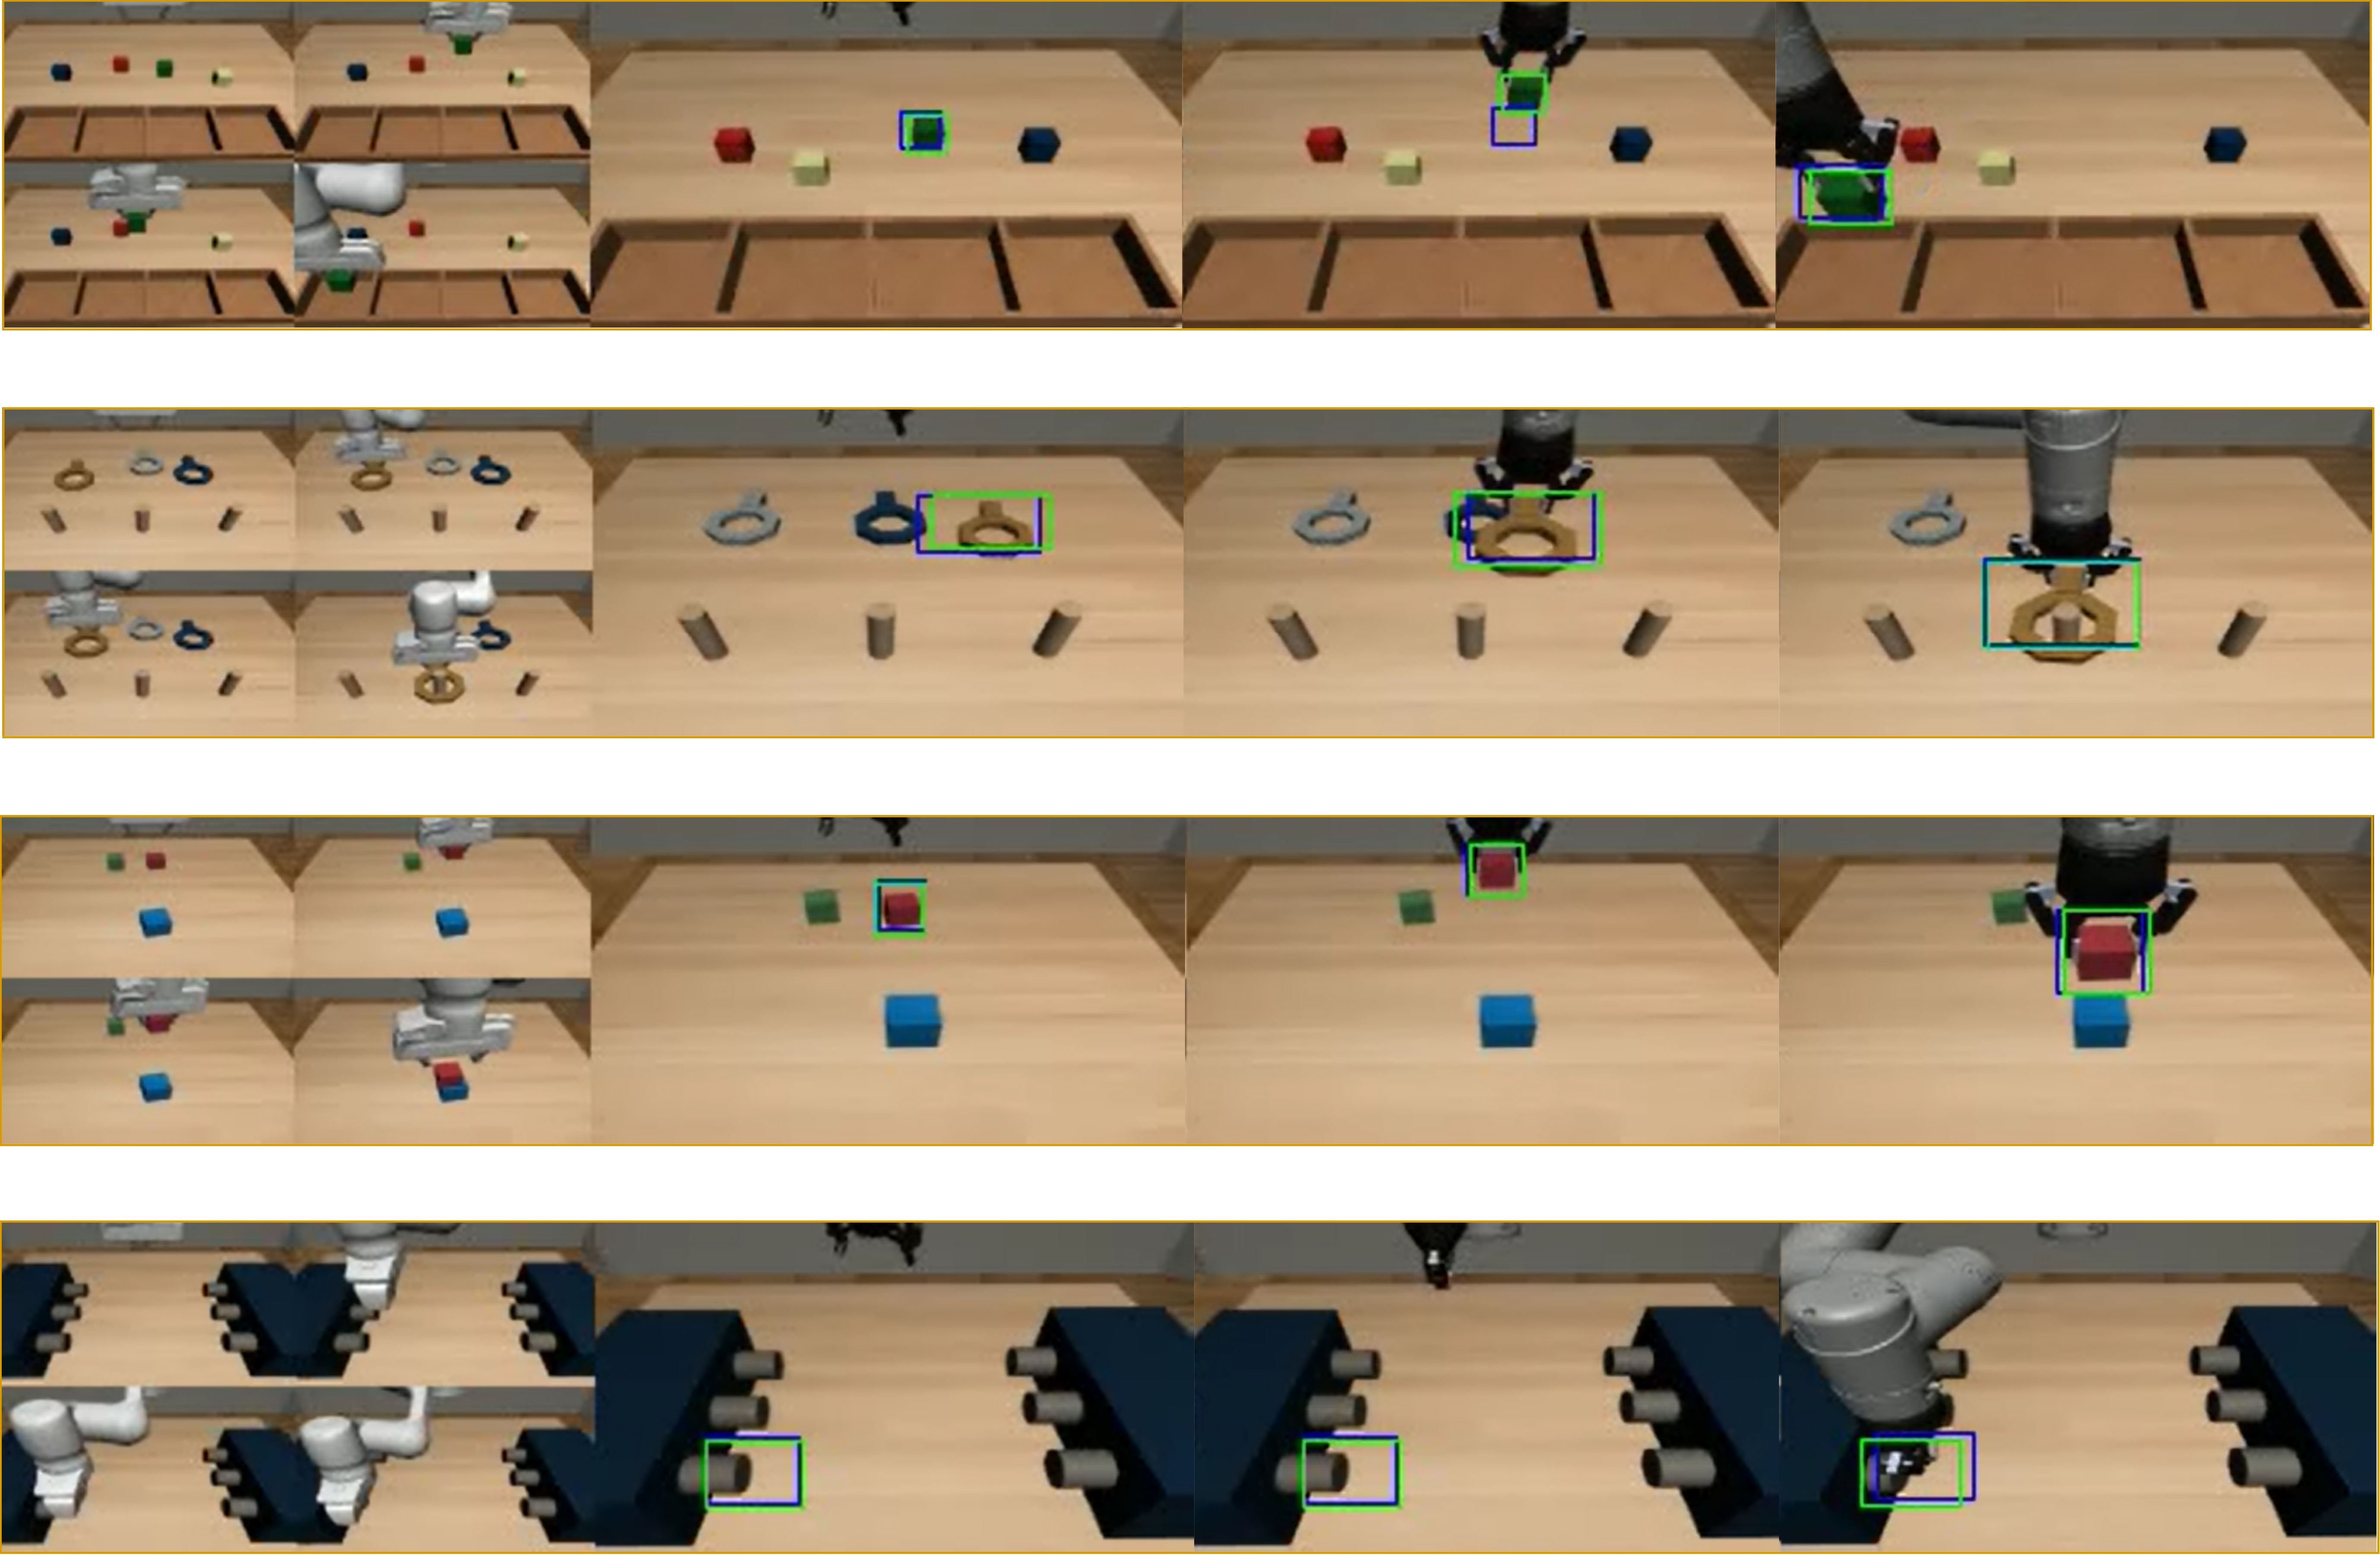
\includegraphics[width=1.0\textwidth]{figures/images/ch2/example_of_prediction_ctod_single.jpg}
    \caption{Example of predictions generated by the CTOD module in the single-task scenario. The blue-box is the predicted one, while the green is the ground truth.}
    \label{fig:ctod_example_of_prediction}
\end{figure}


\paragraph*{Multi-task multi-variation scenario}\mbox{}\\
In the multi-task multi-variation scenario, a single model was trained to perform all four tasks. This setup enables a more rigorous validation of the COD module in a complex environment, where objects of different shapes and sizes are involved across various tasks. Table \ref{table:ctod_multi_task_performance} presents the overall performance of the COD module in terms of Precision and Recall. In this scenario, the system consistently generates bounding boxes for the "target" class (achieving a Recall of 1.00 for all tasks) with an average overlap greater than 0.5. A similar trend as in the single-task scenario is observed, with a lower Precision for the Pick-Place task due to the same reasons previously explained.

Furthermore, compared to the single-task setting, a slight reduction in Average IoU is observed, which can be attributed to the increased complexity of the task. In this multi-task scenario, a single Fast R-CNN must predict bounding boxes across a diverse set of manipulation tasks, where objects may be similar but appear at different scales in the input images. This variation adds further complexity to the prediction process.


\subsubsection{Target object and final position detector}
\label{sec:cod_tofpd}
This set of validation tests focuses on training the COD module in the complete scenario described in Section \ref{sec:cod_problem}. In this setting, the COD module is trained to predict bounding boxes for both the target object and the final location of interest. Specifically, for the three tasks involving the ``pick-and-place" primitive (i.e., Pick-Place, Nut-Assembly, and Stack-Block), the final location corresponds to the target bin, peg, and block to be stacked, respectively. In contrast, for the Press-Button task, the target location is defined as the bounding box of the initial button, translated to the final position of the pressed button (Figure \ref{fig:press_button_target_placing}).
\begin{figure}[t]
    \centering
    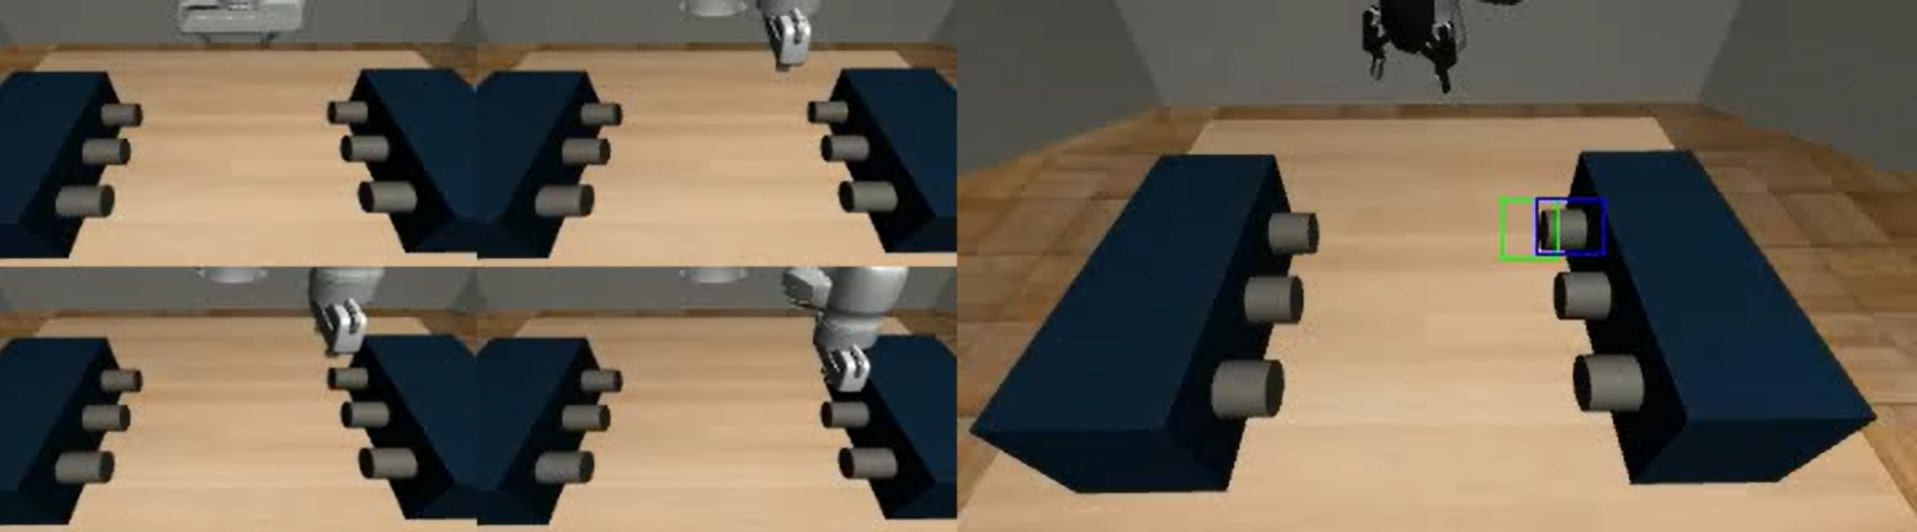
\includegraphics[width=0.9\textwidth]{figures/images/ch2/press_button_target_placing.jpg}
    \caption{Example of Target Bounding Box and Final Placing Position Definition for the Press-Button Task. In this task, the target bounding box is represented by the green bounding box, which encloses the button that needs to be pressed. The blue bounding box represents the final placing position, indicating the location where the robot's end-effector should be positioned to successfully press the button.}
    \label{fig:press_button_target_placing}
\end{figure}


\begin{table}[t]
    \centering
    \caption{Results of the COD module obtained in the single-task multi-variation scenario. Performances are reported in terms of \textit{Precision} (Prec), \textit{Recall} (Rec) with an IoU threshold of 0.5 and the Average IoU $(IoU_{avg})$ for both the bounding-box of the ``target" and the ``target-place" classes.}
    \label{table:cod_single_task_performance}
    \resizebox{\linewidth}{!}{%
    \begin{tabular}{|c|c|c|c|c|} 
    \hline
    \textbf{Task} & \textbf{Precision@0.5} & \textbf{Recall@0.5} & \begin{tabular}[c]{@{}c@{}}$\mathbf{IoU_{avg}}$~\\(target)\end{tabular} & \begin{tabular}[c]{@{}c@{}}$\mathbf{IoU_{avg}}$~\\(target-place)\end{tabular} \\ 
    \hhline{|=====|}
    Pick-Place & 0.667 & 1.00 & 0.374 & 0.826 \\ 
    \hline
    Nut-Assembly & 0.958 & 1.00 & 0.705 & 0.909 \\ 
    \hline
    Stack-Block & 0.979 & 1.00 & 0.787 & 0.827 \\ 
    \hline
    Press-Button & 0.967 & 1.00 & 0.799 & 0.683 \\
    \hline
    \end{tabular}
    }
    \end{table}
% \begin{table}[t]
%     \centering
%     \refstepcounter{table}
%     \caption{Distribution of the predicted bounding boxes generated by the CTOD module in the single-task, multi-variation scenario.}
%     \label{table:ctdo_single_task_prediction_distribution}
%     \resizebox{\linewidth}{!}{%
%     \begin{tabular}{|c|c|c|c|c|c|} 
%     \hline
%     \textbf{Task} & \textbf{TP} & \begin{tabular}[c]{@{}c@{}}\textbf{FP }\\\textbf{pre-picking}\end{tabular} & \begin{tabular}[c]{@{}c@{}}\textbf{FP }\\\textbf{post-picking}\end{tabular} & \begin{tabular}[c]{@{}c@{}}\textbf{FN }\\\textbf{pre-picking}\end{tabular} & \begin{tabular}[c]{@{}c@{}}\textbf{FN }\\\textbf{post-picking}\end{tabular} \\ 
%     \hhline{|======|}
%     \begin{tabular}[c]{@{}c@{}}Pick-Place \\(XXXX)\end{tabular} & XXXX & XXXX & XXXX & XXXX & XXXX \\ 
%     \hline
%     \begin{tabular}[c]{@{}c@{}}Nut-Assembly \\(XXXX)\end{tabular} & XXXX & XXXX & XXXX & XXXX & XXXX \\ 
%     \hline
%     \begin{tabular}[c]{@{}c@{}}Stack-Block\\(XXXX)\end{tabular} & XXXX & XXXX & XXXX & XXXX & XXXX \\ 
%     \hline
%     \begin{tabular}[c]{@{}c@{}}Press-Button\\(XXXX)\end{tabular} & XXXX & XXXX & XXXX & XXXX & XXXX \\
%     \hline
%     \end{tabular}
%     }
%     \end{table}

\begin{table}[t]
    \centering
    \caption{Results of the COD module obtained in the multi-task multi-variation scenario. Performances are reported in terms of \textit{Precision} (Prec), \textit{Recall} (Rec) with an IoU threshold of 0.5 and the Average IoU $(IoU_{avg})$ for both the bounding-box of the ``target'' and the ``target-place'' classes.}
    \label{table:cod_multi_task_performance}
    \resizebox{\linewidth}{!}{%
    \begin{tabular}{|c|c|c|c|c|} 
    \hline
    \textbf{Task} & \textbf{Precision@0.5} & \textbf{Recall@0.5} & \begin{tabular}[c]{@{}c@{}}$\mathbf{IoU_{avg}}$ \\~(target)\end{tabular} & \begin{tabular}[c]{@{}c@{}}$\mathbf{IoU_{avg}}$~\\(target-place)\end{tabular} \\ 
    \hhline{|=====|}
    Pick-Place & 0.735 & 1.00 & 0.457 & 0.825 \\ 
    \hline
    Nut-Assembly & 0.951 & 1.00 & 0.685 & 0.898 \\ 
    \hline
    Stack-Block & 0.867 & 1.00 & 0.628 & 0.799 \\ 
    \hline
    Press-Button & 0.925 & 1.00 & 0.734 & 0.687 \\
    \hline
    \end{tabular}
    }
    \end{table}
% \begin{table}[t]
%     \centering
%     \refstepcounter{table}
%     \caption{Distribution of the predicted bounding boxes generated by the CTOD module in the multi-task, multi-variation scenario.}
%     \label{table:ctdo_multi_task_prediction_distribution}
%     \resizebox{\linewidth}{!}{%
%     \begin{tabular}{|c|c|c|c|c|c|} 
%     \hline
%     \textbf{Task} & \textbf{TP} & \begin{tabular}[c]{@{}c@{}}\textbf{FP }\\\textbf{pre-picking}\end{tabular} & \begin{tabular}[c]{@{}c@{}}\textbf{FP }\\\textbf{post-picking}\end{tabular} & \begin{tabular}[c]{@{}c@{}}\textbf{FN }\\\textbf{pre-picking}\end{tabular} & \begin{tabular}[c]{@{}c@{}}\textbf{FN }\\\textbf{post-picking}\end{tabular} \\ 
%     \hhline{|======|}
%     \begin{tabular}[c]{@{}c@{}}Pick-Place \\(XXXX)\end{tabular} & XXXX & XXXX & XXXX & XXXX & XXXX \\ 
%     \hline
%     \begin{tabular}[c]{@{}c@{}}Nut-Assembly \\(XXXX)\end{tabular} & XXXX & XXXX & XXXX & XXXX & XXXX \\ 
%     \hline
%     \begin{tabular}[c]{@{}c@{}}Stack-Block\\(XXXX)\end{tabular} & XXXX & XXXX & XXXX & XXXX & XXXX \\ 
%     \hline
%     \begin{tabular}[c]{@{}c@{}}Press-Button\\(XXXX)\end{tabular} & XXXX & XXXX & XXXX & XXXX & XXXX \\
%     \hline
%     \end{tabular}
%     }
%     \end{table}
\paragraph*{Single-task multi-variation scenario}\mbox{}\\
Table \ref{table:cod_single_task_performance} summarizes the performance of the COD module in the single-task, multi-variation evaluation setting. It can be observed that, even in this scenario, the COD module consistently identifies both the target object and the target placement location. Specifically, the average Intersection over Union ($IoU_{avg}$) is generally higher for the target-placement class. This is because, for the Pick-Place, Nut-Assembly, and Stack-Block tasks, the placement location is fixed, making the detection problem easier for the conditioning module to address. 

Regarding the ``target" class, the $IoU_{avg}$ is lower compared to Table \ref{table:ctod_single_task_performance}, with a significant drop observed in the Pick-Place task. However, by examining the distribution of false positives, it can be noted that, out of \textbf{7565} false-positive cases, \textbf{2001} occurred during the reaching phase, while the remaining \textbf{5564} occurred during the placing phase. 

It is worth noting that the module can still identify the region of the target object. In fact, by lowering the IoU threshold to 0.1, the number of false positives during the reaching phase drops to 155, indicating that the system is able to detect the region of interest, albeit with lower precision. Nevertheless, for the task at hand, having consistently precise bounding boxes is not critical, as the control module is designed to be robust against minor errors or imprecision in bounding box predictions.


\paragraph*{Multi-task multi-variation scenario}\mbox{}\\
The final evaluation setup largely confirms the trends observed in the previous experiment. Table \ref{table:cod_multi_task_performance} presents the results from the COD module trained in the multi-task scenario. A slight decrease in Precision is again noted, corresponding to a reduction in $IoU_{avg}$. This decrease can be attributed to the same factors discussed in the earlier multi-task setup, with the added complexity of the module needing to predict the bounding box for the target placement location.

Interestingly, this trend differs slightly for the Pick-Place task. In this case, $Precision@0.5$ improves by $+0.068$ from the Single-Task (Table \ref{table:cod_single_task_performance}) to the Multi-Task (Table \ref{table:cod_multi_task_performance}) scenario, driven by an $IoU_{avg}$ increase of $+0.083$, for the \textit{target} class. Overall, this improvement has a limited impact on the system accuracy in detecting the target object during the motion phase. Specifically, among the \textbf{6036} false positives (1529 fewer than in the single-task scenario), \textbf{1187} occurred during the reaching phase (814 fewer than in the single-task scenario), while the remaining \textbf{4849} (715 fewer than in the single-task scenario) occurred during the placing phase. These results indicate that the system shows slightly improved precision in bounding box prediction during the reaching phase, though it continues to encounter challenges during the placing phase.


% In conclusion, this paragraph has introduced the COD module, a Conditioned-Convolutional Neural Network designed to address a novel object-detection problem. The module predicts category-agnostic bounding boxes for the two key regions in a manipulation task: the region where the object to be manipulated is located and the final region where the task is completed (e.g., placing the box, assembling the nut, stacking the block, or pressing the button). In a highly generalized multi-variation scenario, where the object position is not predefined, and the semantic attribute assigned to the object is dynamically specified by a command, which is given through a video demonstration of another agent performing the desired task.


% The results demonstrate that the proposed module effectively handles both single-task and multi-task scenarios, generating bounding boxes that are correctly classified and accurately identify the regions of interest.

% In Chapter \ref{ch:occp}, it will be shown how the positional information from this command can be effectively utilized to inform the control module about the regions of interest, addressing the problem of target misidentification.
